\documentclass[ letterpaper, titlepage, fleqn]{article}

\usepackage[utf8]{inputenc}
\usepackage[slovene]{babel}
\usepackage[margin=60px]{geometry}
\usepackage{amsmath}
\usepackage{amssymb}
\usepackage{enumerate}
\usepackage{graphicx}
\setlength\parindent{0pt}

\begin{document}

\title{$\sigma$-irregularity vs. total $\sigma$-irregularity}
\author{Nejc Ševerkar \& Anja Trobec}
\date{\today}
\maketitle
\pagebreak

\thispagestyle{empty}
\tableofcontents
\pagebreak

\section{Uvod}
V projektni nalogi se bova ukvarjala z merjenjem iregularnosti enostavnih neusmerjenih grafov z
dvema na videz podobnima metodama, {\em $\sigma$-irregularity} in {\em total $\sigma$-irregularity},
definiranima kot 
$$
\sigma(G) = \sum_{(u, v) \in E(G)}(d_u - d_v)^2 
\quad \text{in} \quad
\sigma_t(G) = \sum_{(u, v) \in V(G)}(d_u - d_v)^2
$$
Cilj naloge je maksimizacija razmerja, definiranega kot 
$$\sigma_r(G) = \frac{\sigma_t(G)}{\sigma(G)}$$
pri danem redu grafa $n \in \mathbb{N}$ in tako ugotoviti 
stopnjo naraščanja $\sigma_r(G)$, v odvisnosti od reda.

Ker nas grafi, za katere to razmerje ni definirano,
torej v primeru $\sigma(G) = 0$, ne zanimajo, definiramo $\sigma_r(G) = 0$.
To je natanko tedaj, kadar so vse komponenete grafa $G$ regularne.

\subsection{Naloge}

Najina glavna naloga je torej poiskati maksimalno razmerje $\sigma_r(G)$ med grafi na $n$
vozliščih in jih temeljito preučiti. Najprej bova to počela za majhne grafe, potem pa bova 
z algoritmi problem reševala še za grafe reda $n$. \\

Po prvih oprijemljivih ugotovitvah naju čakajo naslednje naloge. \\

Za optimalne grafe je dana hipoteza, da so krajišča njihovih povezav vedno na absolutni razliki $1$. \\
To bova preverila tako, da bova izračunala število vozlišč za katera
to ne velja pri vsakem optimalnem grafu in ta prikazala z grafom. \\

Naslednja stvar, ki pa jo bova morala preveriti je ta, da je sup$$\frac{\sigma_t(G)}{\sigma(G)}$$ 
reda $O(n^2)$. 
Poiskati bova morala še ustrezno konstanto $c$ s katero bo aproksimacija $cn^2$ najustreznejša.

\section{Osnovna Teorija}

\subsection{Maksimalna Stopnja Naraščanja}
Ker bomo za analizo in primerjavo potrebovali zgornjo mejo stopnje naraščanja
zaporedja $(\max(\sigma_r(G_n)))_n$ v odvisnosti od reda $n$ si poglejmo 
naslednji račun.
$$
\sigma_r(G) = \frac{\sigma_t(G)}{\sigma(G)} 
\leq \sigma_t(G)
= \sum_{(u, v) \in V(G)}(d_u - d_v)^2 
< \sum_{(u, v) \in V(G)}n^2
< n^2  n^2 = n^4,
$$
Sledi, da je red naraščanja $O(n^4)$.

\subsection{Nepovezani Grafi}
Ker sva opazila, da družina nepovezanih grafov doseže maksimalno stopnjo naraščanja,
se lahko po konstrukciji družine takšnih grafov $G_n$ za $\forall n \in \mathbb{N}$
osredotočimo samo na povezane grafe.
\\\\
Konstrukcije grafov $G_n$, za katere ima zaporedje $(\max(\sigma_r(G_n)))_n$ stopnjo 
naraščanja $O(n^4)$ je sledeča.
Vzamemo $n / 2$ vozlišč in iz njih konstruiramo poln graf
medtem, ko v preostalih $n /2$ vozliščih povežemo 3 vozlišča z dvema povezavama.
Po kratkem premisleku lahko formuliramo naslednjo neenakost.
$$\sigma_r(G_{2n}) > \frac{(n - 3)n \binom{n}{2}}{2} = \frac{(n - 3)n n(n - 1)}{4} = \Theta(n^4)$$.
\\
S tem sva zaključila preučevanje nepovezanih grafov.

\section{Ideja Iskanja Optimalnih Grafov}
Problem bova reševala v Pythonu in si občasno pomagala s knjižnjico Networkx,  
s katerim bodo grafično predstavljeni grafi.

\subsection{Metahevristike}
Za optimalno vrednost $\sigma_r$ na grafih reda $n$ morava testirati vse neizomorfne
grafe tega reda, katerih je $\Omega(2^n)$. Če upoštevamo, da izračun $\sigma_r(G)$ 
zahteva $\Omega(n^2)$ operacij, dobimo skupno časovno zahtevnost $\Omega(n^2 2^n)$.
Očitno ta zahtevnost predstavlja problem že za grafe reda $10$, 
torej bova morala poiskati alternativni pristop v obliki metahevrističnih algoritmov. \\

Ideja bo torej sistematično postopati po prostoru povezanih enostavnih grafov reda $n$ in 
tako iskati aproksimacijo grafa $G$, ki maksimizira vrednost $\sigma_r$ na tem prostoru.

Za učinkovito delovanje teh procesov pa potrebujemo definirati ustrezno topologijo 
na prostoru, torej podati pojem bližine, saj jo zahteva večina hevrističnih algoritmov.

To bova naredila v obliki zaporednega dodajanja ali odstranjevanja naključnih povezav v 
danem grafu, pri čimer morava paziti, da ohranjava povezanost grafa, 
torej z drugimi besedami ne odstraniva mostov.\\
Za te namene je napisana knjižnjica, ki poda podporo za izbiro teh povezav
in splošno generiranje naključnih povezanih grafov.

\subsection{Simulated Annealing}
Eden od algoritmov, ki naj bi rešil ta problem je {\em Simulated Annealing}, 
katerega implementacija je končana, a brez okolice, ki bi vrnila dobre rezultate.
Iz tega razloga sva poskusila implementacijo drugega algoritma.

\section{Reševanje Problema}

\subsection{Majhni grafi}
Za majhne grafe sva na strani ** našla že generirane povezane neizomorfne grafe do stopnje 9.
Na njih sva poiskala maksimalne $\sigma_r(G)$, ki so zapisane v naslednji tabeli.

\begin{center}
    \begin{tabular}{|  l | c | }
      \hline
      $n$ & $\sigma_r(G)$ \\ \hline
      2 & 0 \\ 
      3 & 1 \\ 
      4 & 3 \\ 
      5 & 3 \\ 
      6 & 5 \\ 
      7 & 13 \\ 
      8 & 19 \\ 
      9 & 14.5 \\ 
      \hline
    \end{tabular}
\end{center}

Grafov na večjemu številu vozlišč je preveč za posamično analizo, torej
se lotimo implementacije {\em Simulated Annealing} algoritma.

\subsection{Večji grafi}

Med večjimi grafi bomo optimume iskali s pomočjo algoritma
{\em Simulated Annealing}. Ta sprejme 3 argumente: število vozlišč, število simulacij
in definicijo okolice grafa.

Okolice so lahko poljubne in se delijo na lokalne in globalne.
Lokalne okolice spreminjajo graf po povezavah, globalne pa
konstruirajo nov graf, ki ima morda kakšne podobne karakteristike kot prejšnji.

Izkazalo se je da aplikacija samo lokalnih okolic ni dovolj pri velikih grafih in sva zato
iskanje izvedla v dveh delih. Prvi del je klicanje SA na globalni okolici, nakar
pa še na lokalni, saj ta naredi na tem male optimizacije, ki jih globalne spremembe 
niso bile zmožne doseči.

Lokalno izboljšavanje nastopi v obliki minimizacije $\sigma(G)$ z osredotočanjem na
povezave, kjer je razlika med $d_G(V)$ in $d_G(U)$ za neka $uv \in E(G)$ največja.

Po nekaj testih je začela biti očitna struktura optimalnih grafov in sicer
njihova oblika je sestavljena iz dveh delov. V prvem nastopa polni podgraf, 
na drugem pa so povezave redke in je zato podgraf blizu drevesu, kot lahko 
vidimo na spodnji sliki grafa na 20ih vozliščih. \\
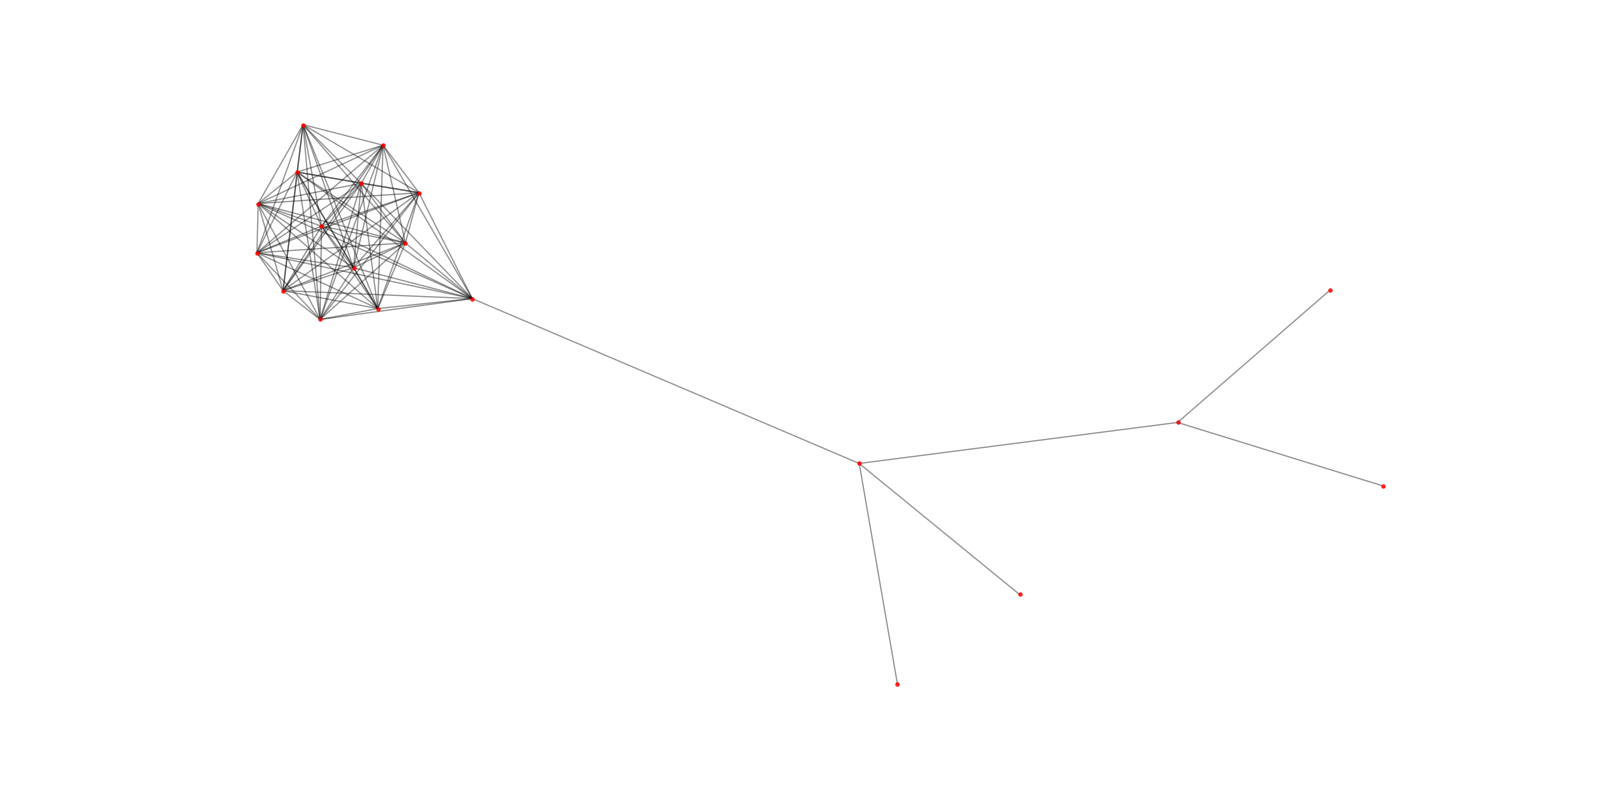
\includegraphics[width=\textwidth, height=8cm]{sample.png} \\
Ta sestava je primerna, saj razlike med polnim grafom in redkim prispevajo 
k vrednosti $\sigma_t$, medtem ko vrednost $\sigma$ ostaja enaka, saj so v obeh
delih grafa sosednje povezave podobnih stopenj. To je skoraj res, a naletimo na posebno povezavo,
ki je prisotna v teh grafih in to je most med polnim in praznim podgrafom. Brez te povezave
bi imeli stopnjo naraščanja $O(n^4)$, a njena prisotnos znatnot povišuje vrednost $\sigma$.

Naš problem se po tej analizi prevede v to kako zvezno, torej s čim manjšo razliko stopenj sosednih povezav, 
povezati poln podgraf z redkim.

\subsection{Distribucija stopenj vozlišč}
Narisala bova graf na katerem bosta za graf $G$ velikosti $n$ izpisani
vrednosti $\sigma_r(G)$ in $\max_{v \in V(G)}d_G(v)$ na katerem
se bo lepo videla korelacija.

\subsection{Kvadratična stopnja naraščanja}
Preveriti morava še, če je stopnja narašanja zaporedja
$(\max(\sigma_r(G_n)))_n$, kjer $G_n$ graf stopnje $n \in \mathbb{N}$,
$O(n^2)$ in poiskati ustrezno konstanto $c \in \mathbb{R}$, ki 
se naraščanju najbolj prilega.
\\\\
Predpostavimo, da smo optimum izračunali za $n$ grafov in
označimo $X(n, p) = (1^p, 2^p, \dots, n^p)^T \in \mathbb{R}^{nx1}$ 
in $a = (a_1, a_2, \dots, a_n)^T$ vektor, kjer $a_i$ predstavlja
dobljeni optimalni $\sigma_r(G_i)$ za graf $G_i$ na $i$ vozliščih.
Problem pri danem $p \in \mathbb{R}^{+}$ zahteva rešitev linearnega sistema 
$$cX(n, p) = a.$$
Ta sistem seveda ne bo rešljiv, iskanja aproksimacije pa se bomo
lotili z metodo najmanjših kvadratov, torej minimum $2$-norme
razlike obeh strani bo dosežen pri
$$c = ||X(n, p)||_{2}^2 / <a, X(n, p)>.$$

Najboljšo aproksimacijo naraščanja $\sigma_r$ bomo poiskali 
z diskretizacijo $D \subset [0, 4]$ in za $\forall p \in D$ 
izračunali prej definirani $c$, na koncu pa izbrali tisto kombinacijo
$(c, p)$, za katero je $||cX(n, p) - a||_{2}$ najmanjši.
\\\\
Tako dobimo po testiranju na vozliščih od $3$ do $700$ naslednji graf.\\
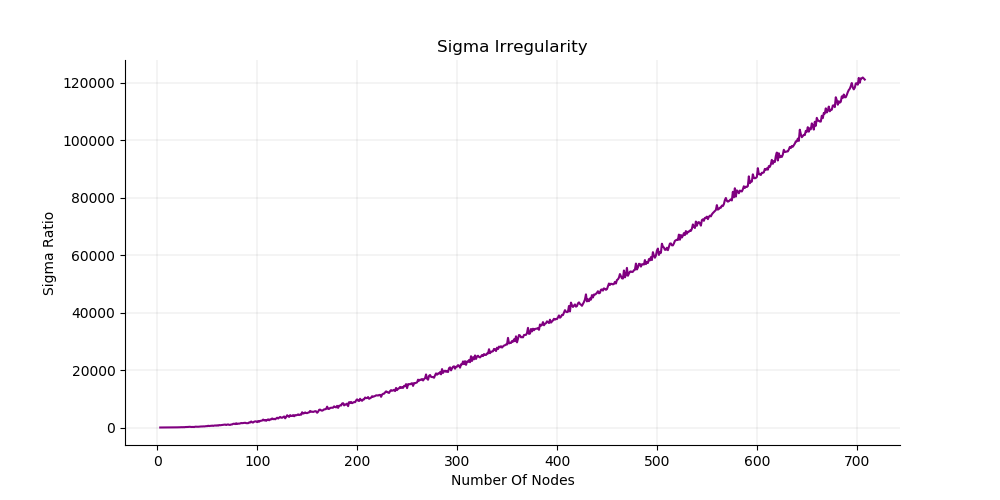
\includegraphics[width=\textwidth, height=8cm]{raw_graph.png} \\
Po prej opisani metodi dobimo par $(c, p)$, za katerega $cn^p$ najbolje opisuje
$\sigma_r$ naraščanje. Ta par je izračunan kot $(0.19319714558507617, 2.0360000000000014)$ in
njegova aproksimacija naraščanja je prikazana na naslednjem grafu.\\
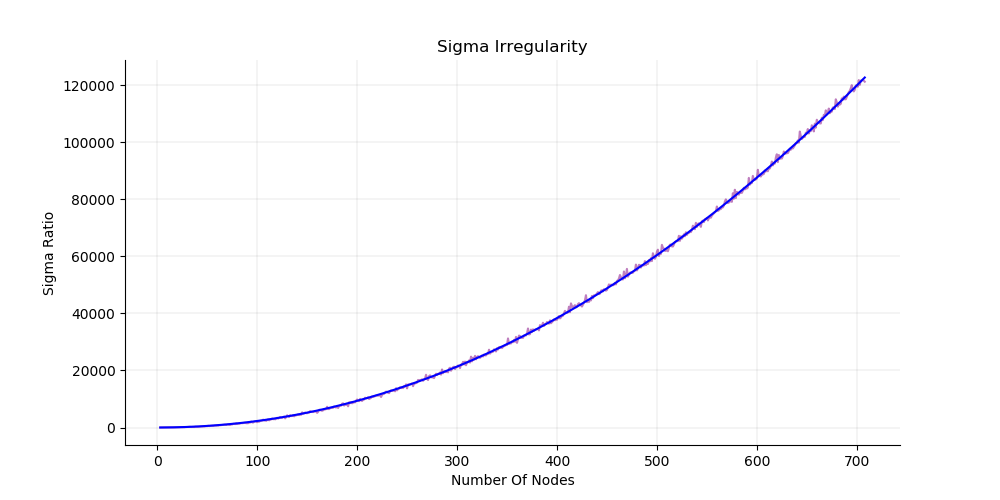
\includegraphics[width=\textwidth, height=8cm]{aproximation_graph.png}\\

\subsection{Opisi Implementiranih Algoritmov}
Podali bomo kratek opis vseh vključenih algoritmov v napisani knjižnici in njihovo časovno zahtevnost.
V tabeli bo $n$ označeval število vozlišč grafa, $m$ pa število povezav.
\begin{center}
    \begin{tabular}{ l  l  l}
      Ime & Opis & T \\ 
      {\em sigma} & izračuna vrednost $\sigma(G)$ na danem grafu $G$ & $O(n + m)$ \\
      {\em sigma\_t} & izračuna vrednost $\sigma_t(G)$ na danem grafu $G$ & $O(n^2)$ \\
      {\em sigmaRatio} & izračuna vrednost $\sigma_r(G)$ na danem grafu $G$ & $O(n^2)$ \\
      {\em sigmaUpdate} & izračuna razliko $\sigma$ po odstranjeni ali dodani povezavi v $G$ & $O(n)$ \\
      {\em sigmaArgmax} & vrne povezavo, ki maksimizira $\sigma$ vrednost v danem grafu $G$ & $O(n + m)$ \\
      {\em randomConnectedGraph} & konstruira naključni graf na $n$ vozliščih &  $O(n^2 \log^*(n))$ \\ 
      {\em  randomTree} & konstruira naključno drevo na $n$  vozliščih & $O(n)$ \\
      {\em randomPath} & konstruira naključno pot na $n$ vozliščih & $O(n)$ \\
      {\em randomSubtree} & poišče naključno poddrevo danega grafa & $O(n)$ \\
      {\em randomSigmaOptAprox} & konstruira graf, ki naj bi bil grob približek optimalnemu & $O(n^2)$ \\
      {\em nonBridges} & poišče $k$ povezav, ki niso mostovi v danem grafu & $O(m + n)$ \\
      {\em nonEdges} & poišče $k$ povezav, ki niso vključene v grafu & $O(n^2)$ \\
      {\em localBasicNeighbor} & graf spremeni z dodajanjem in odstranjevanjem povezav & $O(n^2)$ \\
      {\em globalBasicNeighbor} & uporabi {\em randomConnectedGraph} za konstrukcijo okolice & $O(n^2 \log^*(n))$ \\ 
      {\em globalTwoPartNeighbor} & uporabi {\em randomSigmaOptAprox} za konstrukcijo okolice & $O(n^2)$ \\
      {\em maxSigmaRatio\_annealing} & uporabi Simulated Annealing za iskanje optimalnega grafa & odvisno od argumentov \\
    \end{tabular}
  \end{center}

\end{document}
